
\documentclass[a4paper,11pt]{article}

\usepackage{fontspec}
\setmainfont{Calibri}

\linespread{1}

\setlength{\oddsidemargin}{0cm}
\setlength{\evensidemargin}{0cm}
\setlength{\textheight}{23cm}
\setlength{\textwidth}{16cm}

\usepackage{amssymb,mathrsfs,algorithmic,algorithm,multirow}
\usepackage{amsmath,amsbsy,graphicx,color,url,natbib,tcolorbox}
\usepackage{ccaption}
\setlength{\bibsep}{0.0pt}


\newcommand{\bm}{\mathbf}
\newcommand{\bs}{\boldsymbol}
\newcommand{\mt}{\mathrm}
\newcommand{\nind}{\noindent}

\usepackage{fancyhdr}
\newcommand{\tstamp}{\today}   
\lhead[\fancyplain{}{\rightmark}]       {\fancyplain{}{}}
\rhead[\fancyplain{}{\rightmark}]       {\fancyplain{}{}}
\chead[\fancyplain{}{\centermark}]       {\fancyplain{}{ENGM214 -- Process Modelling and Simulation} }
\pagestyle{fancyplain}

\usepackage{amsthm}
\theoremstyle{definition}
\newtheorem{exmp}{Example}[section]

\title{\vspace{-2cm} Lecture 4 -- Models of lumped parameter systems}

\author{Tao Chen\\
{\small \emph{Department of Chemical \& Process Engineering, University of Surrey, UK}}\\
{\small (email: \texttt{t.chen@surrey.ac.uk}; \hspace{0.5cm} updated on: \today )}
}
\date{}

\begin{document}
\maketitle

%\tableofcontents
\vspace{-0.5cm}

\section{Classification of models and model equation sets}

As has been mentioned in previous lectures, the modelling assumptions and intended use
lead to various model forms. Fig. \ref{fig:model_class} gives a typical classification of process models.
The first factor to consider is spatial variation in system.
If this spatial variation is critical for the intended use of the model, then a distributed parameter model
needs to be developed; otherwise a lumped parameter system is appropriate.
Dynamics refers to whether the variables of interest change with time -- if not, the system is said to be at
``steady-state''. It is worth noting that steady-state is a usual assumption in many design tasks and has
been a centre piece in classic process engineering textbooks. However, for many practical applications
understanding the dynamics is critical.

\begin{figure}[!h]
 \begin{center}
	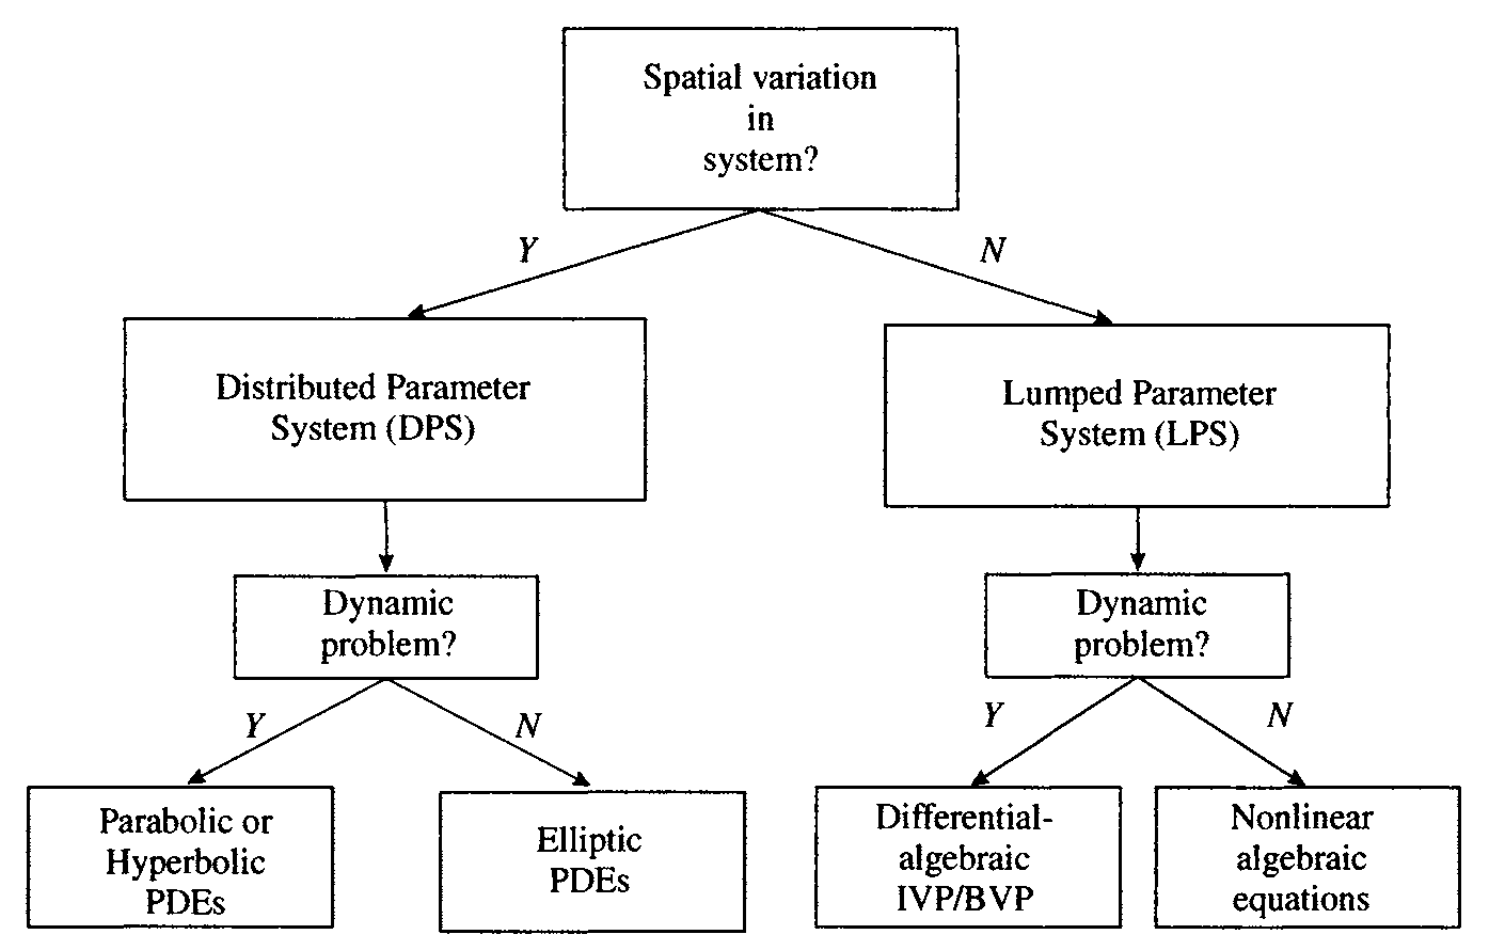
\includegraphics[width=.6\textwidth]{model_class}
 \end{center}
 \caption{Classification of models. PDE: partial differential equation; IVP: initial value problem; BVP: boundary value problem.} 
 \label{fig:model_class}
\end{figure}

A dynamic, distributed parameter system is the most complex discussed in this module, resulting in
partial differential equations as the modelling equations involving time and spatial position.
In contrast, a steady-state lumped parameter system is much simpler giving rise to algebraic equations (can be either linear or non-linear).

\section{Lumped parameter models}

A lumped parameter system has no difference in any properties at different spatial positions
within the \textbf{balance volume}.
Thus no spatial variation of any variable is considered. In addition, there exists no difference 
between different parts of the \textbf{surface}, and thus the position or direction of any boundary-crossing 
flow is not of concern.
Fig. \ref{fig:lump} illustrates the simplification from a general system to a lumped parameter system in terms of the balance volume.

\begin{figure}[!h]
 \begin{center}
	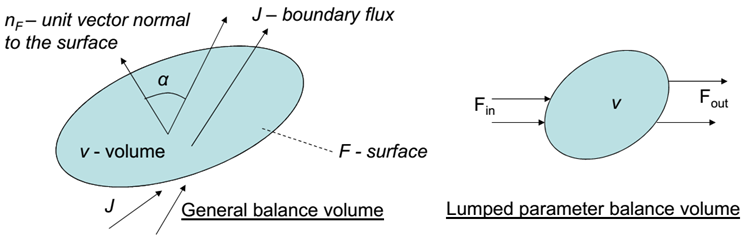
\includegraphics[width=.6\textwidth]{lump}
 \end{center}
 \caption{Illustration of the balance volume of a lumped parameter system.} 
 \label{fig:lump}
\end{figure}

Clearly, lumped parameter systems do not exist in reality but they can be useful models (recall the difference between model and reality discussed in Lecture 1).
Such models can be used to represent systems which are sufficiently well mixed,
or they may represent a relatively homogeneous \emph{part} of a highly heterogeneous system.
This corresponds to the multi-compartmental approach to the modelling of a heterogeneous
system, an alternative to the rigorous approach of distributed parameter systems modelling.
Some examples will be provided to further elaborate these points.

\textbf{Conservation equations.} Recall the general conservation equation in integral form discussed
in Lecture 3, re-written below:
\begin{equation}
	\underbrace{ \frac{d}{d t} \left\{ \int_{\mathcal{V}} \hat{\Phi} (r, t) dv \right\} }_{\substack{ \text{Rate of change of $\Phi$} \\ \text{within volume $\mathcal{V}$} } } 
		\; = \; \underbrace{ -\oint_{\mathcal{F}} J(r,t) \cdot n_{\mathcal{F}}(r) d f }_{\substack{ \text{Net flow of $\Phi$} \\ \text{across the boundary surface $\mathcal{F}$} } }
		\quad + \underbrace{ \int_{\mathcal{V}} \hat{q}(r, t) dv }_{\substack{ \text{Rate of net generation of $\Phi$} \\ \text{within volume $\mathcal{V}$} } }
\end{equation}
\noindent A lumped parameter system has no spatial variation, so each integral term is reduced (or ``lumped'')
to a single variable:
\begin{equation}
	\frac{d \Phi}{d t} = J_C + q, \quad J_C = J_C^{(i)} - J_C^{(o)}
\end{equation} 
\noindent where $J_C^{(i)}$ and $J_C^{(o)}$ represent the inflow and outflow of the conserved extensive quantity, respectively.
We can see the original partial differential equation has been converted into an ordinary differential equation.

Next, we apply the above principle to set up the balance equations for mass, energy and momntum, 
as well as related constitutive relations.

\subsection*{Mass balance}

Conservation of mass with respect to a balance volume is illustrated in Fig. \ref{fig:mass}.
Here we consider a general case with multiple streams of inflow and outflow: $F_j$ [kg s$^{-1}$]
denotes the \emph{total} mass flowrate of inflow stream $j$, and $F_k$ the total mass flow rate of outflow stream $k$.
The total mass within the balance volume is $M$, and its balance equation is:

\begin{equation} \label{eq:mass_total}
	\frac{d M}{d t} = \sum_{j=1}^p F_j - \sum_{k=1}^q F_k
\end{equation}
\noindent where $p$ and $q$ denote the total number of streams of inflow and outflow, respectively.

\begin{figure}[!h]
 \begin{center}
	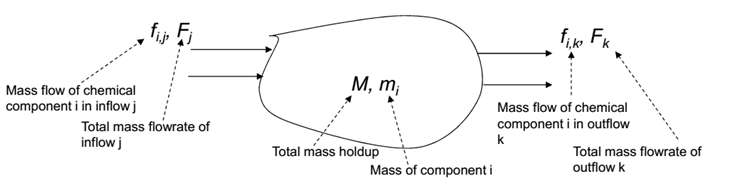
\includegraphics[width=.8\textwidth]{mass}
 \end{center}
 \caption{Illustration of mass balance.} 
 \label{fig:mass}
\end{figure}

In addition to the total mass and total mass flowrate, we are also concerned with those of the chemical species.
For example, within the balance volume there may exist a mixture of two species (components): ethanol and water.
Suppose we have $n$ components, and the corresponding mass balance equations are:

\begin{equation} \label{eq:mass_comp}
	\frac{d m_i}{d t} = \sum_{j=1}^p f_{i,j} - \sum_{k=1}^q f_{i,k} + g_i, \quad i = 1, \ldots, n
\end{equation}
\noindent where $g_i$ [kg s$^{-1}$] is the net generation rate of component $i$ due to reactions.

Note that here the modelling equations are all with respect to \textbf{mass}, which is the fundamental
quantity that is conserved. In some cases especially those involving reactions, it is customery to
express the component mass balance eq. (\ref{eq:mass_comp}) on molar basis,
so that $g_i$ (now on molar basis, [mol s$^{-1}$]) can be further related to the reaction rate $r_i$
and reactor volume $V$ as $g_i = r_i V$; see notes on Lecture 3.
However, when the system involves reactions, care must be taken to express the total mass balance in eq. (\ref{eq:mass_total}) in molar units,
since the total number of moles is not conserved.

\subsection*{Energy balance}

\begin{figure}[!h]
 \begin{center}
	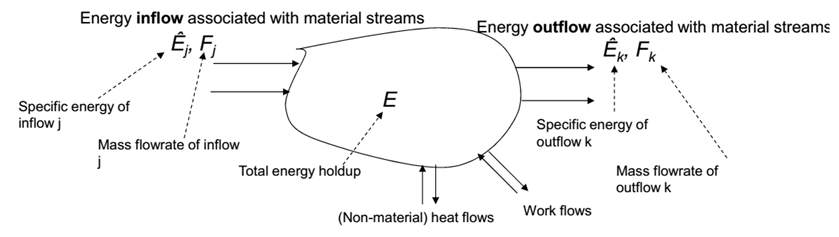
\includegraphics[width=.8\textwidth]{energy}
 \end{center}
 \caption{Illustration of energy balance.} 
 \label{fig:energy}
\end{figure}

Conservation of energy with respect to a balance volume is illustrated in Fig. \ref{fig:energy}.
As far as process modelling is concerned, the total energy in the system $E$ [J] consists of
internal, kinetic and potential energies:
\[
	E = \underbrace{U}_\text{Internal energy} + \underbrace{K_E}_\text{Kinetic energy} + \underbrace{P_E}_\text{Potential energy}
\]
Energy inflow and outflow are associated with the flow of mass. Hence, the amount of energy
in the inflow and outflow streams are expressed in mass-specifc form (i.e. the amount of energy per unit mass):
$\hat{E}_j = (\hat{U} + \hat{K_E} + \hat{P_E})_j$ [J kg$^{-1}$] for inflow and similarly $\hat{E}_k$ [J kg$^{-1}$] for outflow.
As a result, the ``material'' energy flows are given by
\begin{align}
	E_{\textrm{material, in}} &= \sum_{j=1}^p F_j \hat{E}_j = \sum_{j=1}^p F_j (\hat{U} + \hat{K_E} + \hat{P_E})_j \\
	E_{\textrm{material, out}} &= \sum_{k=1}^q F_k \hat{E}_k = \sum_{k=1}^q F_k (\hat{U} + \hat{K_E} + \hat{P_E})_k 	
\end{align}
\noindent The non-material heat flows (e.g. due to conduction, radiation etc.) are collectively
represented by $Q$ (inflow as the positive direction), while the terms relating to work include
shaft work ($W_S$), expansion work $W_E = - \int_{\mathcal{V}} P(r, t) dv $ and
 flow work $W_F = \sum_{j=1}^p F_j (P\hat{V})_j - \sum_{k=1}^q F_k (P \hat{V})_k$:
 \footnote{If these concepts do not seem familiar, refer to \citep{Hangos2001} for details.}
\[
	W = W_S + W_E + W_F
\]

Putting everything together, the general energy balance equation is
\begin{equation} 
	\frac{d E}{d t} = \sum_{j=1}^p F_j \hat{E}_j - \sum_{k=1}^q F_k \hat{E}_k + Q + W
\end{equation}
\noindent which can be re-written by explicitly expressing the ``material'' energy flow and flow work:
\begin{align}
	\frac{d E}{d t} &= \sum_{j=1}^p F_j (\hat{U} + \hat{K}_E + \hat{P}_E)_j 
		- \sum_{k=1}^q F_k (\hat{U} + \hat{K}_E + \hat{P}_E)_k  + Q + W_S + W_E + \sum_{j=1}^p F_j (P\hat{V})_j - \sum_{k=1}^q F_k (P \hat{V})_k \nonumber \\
		&= \sum_{j=1}^p F_j (\hat{U} + P\hat{V} + \hat{K}_E + \hat{P}_E)_j 
			- \sum_{k=1}^q F_k (\hat{U} + P\hat{V} + \hat{K}_E + \hat{P}_E)_k  + Q + W_S + W_E 
\end{align} 
\noindent Notice the relationship between enthalpy ($H$) and internal energy ($U$): $H = U + PV$,
and follow the convention to re-use $W$ to only include shaft and expansion work $W = W_S + W_E$,
the above can be simplified to
\begin{equation} \label{eq:energy}
	\frac{d E}{d t} = \sum_{j=1}^p F_j (\hat{H} + \hat{K}_E + \hat{P}_E)_j 
			- \sum_{k=1}^q F_k (\hat{H} + \hat{K}_E + \hat{P}_E)_k  + Q + W
\end{equation} 

\textbf{Simplified energy balance equations.} The energy balance equation (\ref{eq:energy}) can be simplified
in a number of ways for specific cases.
\begin{enumerate}
	\item \underline{Ignoring kinetic and potential energy terms}. This is realistic for most process systems as their contribution to the 
		overall energy balance is usually small: \\
		\[ \frac{d U}{d t} = \sum_{j=1}^p F_j \hat{H}_j - \sum_{k=1}^q F_k \hat{H}_k  + Q + W \]
	\item \underline{Assuming constant $P$ and $V$}. This is realistic for most liquid phases. Notice $U = H + PV$
		and with constant $P$ and $V$, $d U / d t = d H / d t$, we have: \\
		\[ \frac{d H}{d t} = \sum_{j=1}^p F_j \hat{H}_j - \sum_{k=1}^q F_k \hat{H}_k  + Q + W \]	
	\item \underline{Simplifying the calculation of enthalpies}. Here we usually assume that the properties (e.g. temperature, enthalpy) of the outlet material
		stream are the same as those in the balance volume, i.e. $H = \hat{H}_k, k=1,\ldots,q$.  
		In addition, we assume temperature-independent heat capacity (c.f. Lecture 3) for the inlet material streams (but different inlet streams may have different
		temperature and heat capacity values). These assumption lead to: \\
		\begin{equation} \label{eq:energy2} 
			\frac{d H}{d t} = \sum_{j=1}^p F_j \left[ \hat{H}_j(T) + c_{pj} (T_j - T) \right] - \sum_{k=1}^q F_k \hat{H}(T)  + Q + W
		\end{equation}
		\noindent where $T$ is the temperature of the balance volume, $\hat{H}$ the specific enthalpy of the balance volume;
			$c_{pj}$ and $T_j$ are the specific heat capacity and temperature of inflow material stream $j$.
\end{enumerate}

Eq. (\ref{eq:energy2}) can be combined with the total mass balance equation (\ref{eq:mass_total}), and with several further assumptions,
to give the most common form of energy balance for systems involving reactions:

\begin{equation} \label{eq:energy_react}
	V \rho c_p \frac{d T}{d t} = \sum_{j=1}^p F_j c_{pj} (T_j - T) + r V (-\Delta H_R) + Q + W
\end{equation}
\noindent where $V$ is reactor volume, $\rho$ and $c_p$ the density and specific heat capacity of the balance volume contents,
$r$ the reaction rate and $\Delta H_R$ the heat of reaction. 
\textbf{You should attempt to derive this equation and understand what assumptions have been made, before reading the text box 
at the end of this document.}

\subsection*{Momentum balance}

The momentum balance is described as:
\[
	\left\{\substack{ \textrm{rate of change} \\ \textrm{of momentum} } \right\} = \left\{\substack{ \textrm{rate of momentum} \\ \textrm{into system} } \right\}	 
		- \left\{\substack{ \textrm{rate of momentum} \\ \textrm{out of system} } \right\} + \left\{\substack{ \textrm{rate of momentum} \\ \textrm{generation} } \right\}
\]
\noindent Momentum generation is caused by forces $F_i$ applied to the system. The general balance equation for momentum, $\mathcal M$, is thus:
\begin{equation}
	\frac{d \mathcal M}{d t} = \mathcal M^{(i)} - \mathcal M^{(o)} + \sum_{i=1}^n F_i
\end{equation}

Momentum balance is not normally considered in lumped parameter systems and will not be discussed further.
A full account of momentum balance and transfer is very complex and beyond the scope of this module.
For more details, refer to the classical textbook \citep{Bird2007}.

\vspace{0.8cm}
\textbf{Steady-state models}, by definition, can be obtained by simply setting the differential term in the
left-hand side of the afore-discussed balance equations to zero.

\subsection*{Modelling examples}

\begin{exmp}[A CSTR system]
A well-mixed CSTR with reactant volume $V$ [m$^3$], component mass holdup $m_A$ (in mole units [mol])
for component $A$, feed volumetric flowrate $F^{(i)}$ [m$^3$ s$^{-1}$] with molar concentration
$c_A^{(i)}$ [mol m$^{-3}$], feed temperature $T^{(i)}$ [K], outlet volumetric flowrate 
$F^{(o)}$ [m$^3$ s$^{-1}$], and reaction $A \to P$ with rate
$r_A = k_0 e^{-E/(RT)} c_A$. Furthermore, the physical properties $\rho$ (density) and
$c_p$ (heat capacity) of the feed and reactor contents are assumed to be knon constants.
Heat of reaction $\Delta H_R$ is also a known constant. The system is illustrated in Fig. \ref{fig:cstr}.
\begin{figure}[!h]
 \begin{center}
	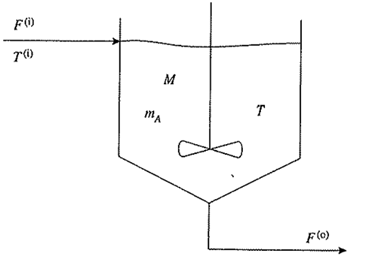
\includegraphics[width=.5\textwidth]{cstr}
 \end{center}
 \caption{Illustration of the CSTR.} 
 \label{fig:cstr}
\end{figure}

By following the principles discussed so far, we first give the conservation equations.
The total mass balance equation is
\[
	\frac{d (\rho V)}{d t} = F^{(i)} \rho^{(i)} - F^{(o)} \rho
\]
and the mass balance for component $A$ in molar units is:
\[
	\frac{d m_A}{d t} = f_A^{(i)} - f_A^{(o)} - V r_A
\]
\noindent where $f_A^{(i)}$ and $f_A^{(o)}$ are the molar flowrate of component $A$ in and out of the tank, respectively.
The energy balance equation, similarly to eq. (\ref{eq:energy_react}), is 
\[
	V \rho c_p \frac{d T}{d t} = F^{(i)} \hat{H}^{(i)} \rho - F^{(i)} \hat{H} \rho - V r_A \Delta H_R
\]
\noindent and the constitutive equations include
\[	f_A^{(i)} = F^{(i)} c_A^{(i)}, \; f_A^{(o)} = F^{(o)} c_A, \; M = V \rho, \; m_A = c_A V \]
\[	r_A = k_0 e^{-E/(RT)} c_A, \; H = M c_p T, \; \hat{H} = H / M, \; \hat{H}^{(i)} = c_p^{(i)} T^{(i)} \]

Finally, we need to specify the initial value for each differential variable:
\[  V(0) = V_0, \; m_A(0) = m_{A_0}, \; T(0) = T_0 \]

\textbf{Food for thought:} Why do we not build a mass balance equation for component $P$, in addition to component $A$?
\end{exmp}


\begin{exmp}[CSTR with jacket for temperature control]
This example will be discussed in Work Session 4.
\end{exmp}


\begin{exmp}[A tea infusion process]
Extraction of active ingredients in tea leaves is an important process to produce tea-based beverage,
which has a huge market worldwide. Fig. \ref{fig:tea} shows a typical experimental set-up to study
this process and the concentration profile in the leaf and solution phases over time.
A mathematical model is to be developed to describe the concentration change over time in the leaf and solution.
\begin{figure}[!h]
 \begin{center}
 	(a)	\hspace{6cm} (b) \\
	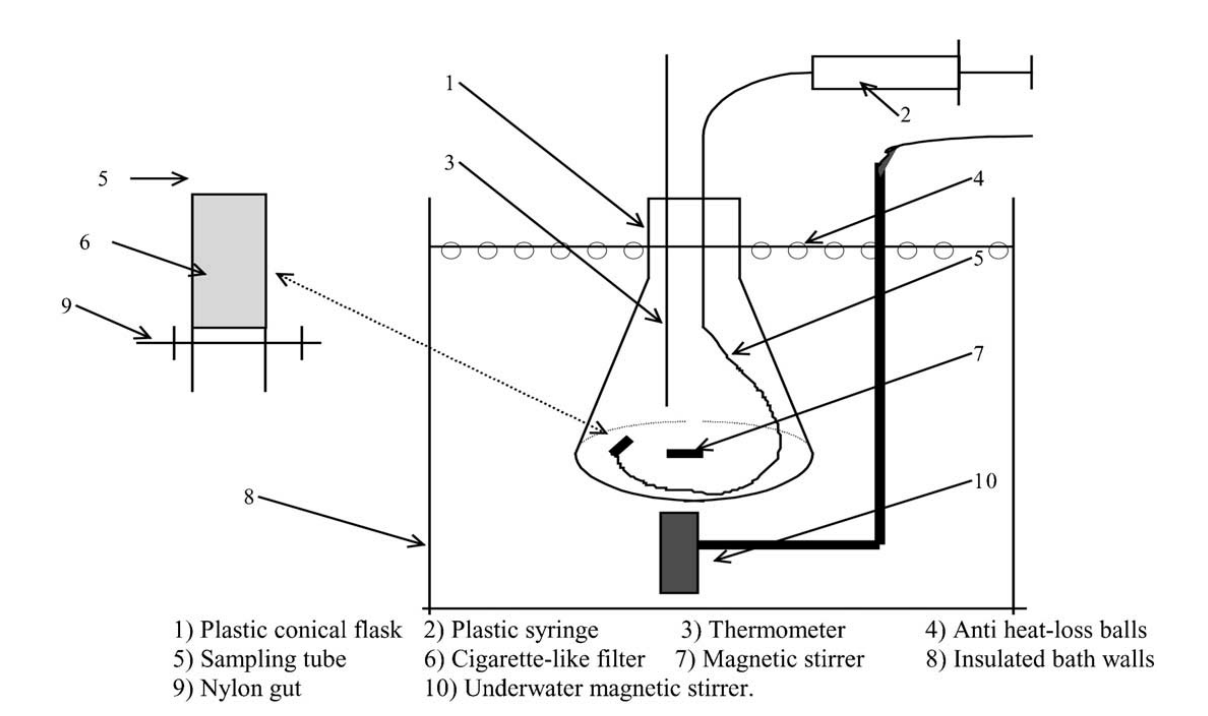
\includegraphics[width=.495\textwidth]{tea}
	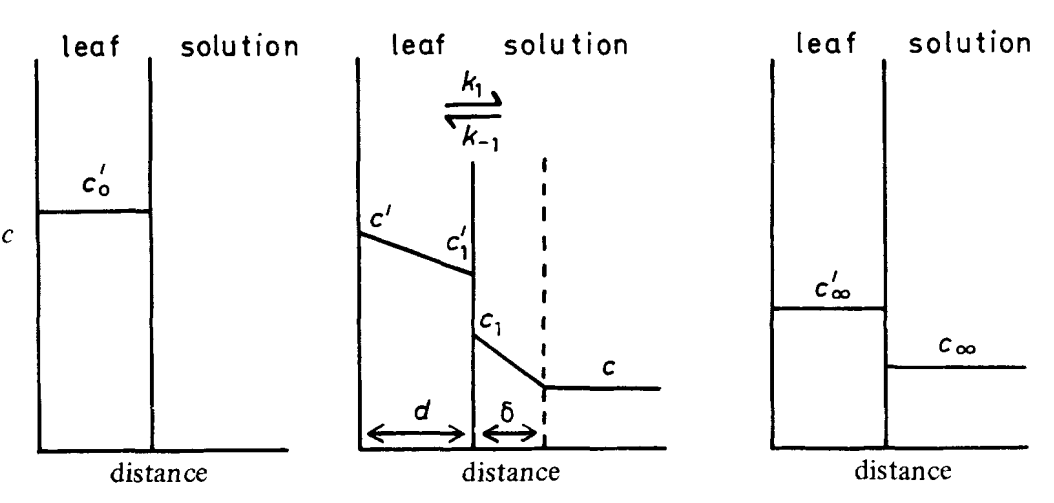
\includegraphics[width=.495\textwidth]{tea_model}	
 \end{center}
 \caption{Illustration of the tea infusion process (a) and the schematic concentration profiles at different times (b).
 	(source: J . Chem. Soc., Furaduy Trans. 1, 1982, 78, 295-305; Food Chemistry 83 (2003) 121–126.} 
 \label{fig:tea}
\end{figure}

We chose a lumped parameter system despite the apparent concentration gradient in the tea leaf,
as illustrated in Fig. \ref{fig:tea}, which is difficult to measure experimentally.
In addition, the main focus is the concentration in solution, which is the product tea beverage, 
and with appropriate stirring in the vessel it's reasonable to assume a uniform concentration of the active ingredients.

The active ingredients extracted from tea can be of many types, such as theaflavins and caffeine.
Here for simplicity we lump them together into a ``pseudo'' aggregate ingredient, whose concentration [kg m$^{-3}$] in
leaf $C_l$ and that in solution $C_s$ are of interest. This is essentially a mass transfer process which has been
briefly discussed in Lecture 3.

Clearly two balance volumes are needed, one for leaf $V_l$ and one for solution $V_s$ [m$^3$].
The mass balance equations are:
\begin{align}
 	\textrm{solution phase:} \quad & V_s \frac{d C_s}{d t} = A k_s ( K C_l - C_s) \\
	\textrm{leaf phase:} \quad & V_l \frac{d C_l}{d t} = - A k_s ( K C_l - C_s)	
\end{align}
\noindent where $A$ [m$^2$] is the interfacial area for mass transfer, $k_s$ is the mass transfer
coefficient and $K$ is the ``partition coefficient'' defined as the ratio of the concentration in
solution to the concentration in leaf at \emph{equilibrium}:
\[
	K = \frac{ C_{s, equ} }{ C_{l, equ} }
\]
\noindent which can be experimentally determined from equilibrium experiments.
The initial conditions need to be given: $C_s(0) = C_{s,0}$ and $C_l(0) = C_{l,0}$.
If the other parameters can be obtained through experiments and measurement,
including $V_s$, $V_l$ and $A k_s$, the model can be solved to predict
the dynamics of concentrations.

\end{exmp}


\section{General form of dynamic models}

In general, a dynamic model of a lumped parameter system is a differential-algebraic equation (DAE)
system which contains three parts:

\begin{align}
	\frac{d x}{d t} = f(x, y, t),  \; &\leftarrow \; \textrm{A set of ODEs} \\
	g(x, y, t) = 0,                     \; &\leftarrow \; \textrm{A set of algebraic equations} \\
	x(0) = x_0                          \; &\leftarrow \; \textrm{A set of initial conditions}
\end{align}

\noindent where $x$ is a set of ``state'' or ``differential'' variables, and $y$ is a set of algebraic variables.
The methods to solve these equations will be discussed in detail in Lecture 5.
Here briefly, given a set of initial conditions, the algebraic equations can be solved first
to obtain the values of (unknown) algebraic variables ($y$) at time $t=0$. 
Values of all the algebraic variables as well as the initial conditions will then allow the evaluation of $f(x(0), y(0), t=0)$, based on which the ODEs can be numerically integrated.
For this approach to work, there are two issues that need to be considered.

\textbf{The issue of consistent initial conditions.} This is best explained through an example. Consider an DAE system below with two differential variables ($x_1$, $x_2$)
and one algebraic variable $z_1$:
\begin{align}
	\frac{d x_1}{d t} &= x_1 + x_2 + z_1 \label{eq:init1} \\
	\frac{d x_2}{d t} &= x_1 - x_2 - z_1 \label{eq:init2} \\
	0 &= x_1 + 2 x_2 - z_1 \label{eq:init3} 
\end{align}
\noindent For this DAE system in eqs. (\ref{eq:init1})(\ref{eq:init2})(\ref{eq:init3}),
we can set the initial conditions, $x_1(0)$ and $x_2(0)$, to any value, and solve
$z_1(0)$ from eq. (\ref{eq:init3}), and then use a numerical integration method in Lecture 5 to solve this system. In other words, there is no constraint on the initial conditions of the DAE system in eqs. (\ref{eq:init1})(\ref{eq:init2})(\ref{eq:init3}).

Now replace the algebraic equation  (\ref{eq:init3}) with
\begin{equation} \label{eq:init4}
	0 = x_1 + 2 x_2
\end{equation}
\noindent which defines a different DAE system with eqs. (\ref{eq:init1})(\ref{eq:init2})(\ref{eq:init4}). Clearly eq. (\ref{eq:init3}) puts constraint on $x_1$ and $x_2$:
 for initial conditions only of $x_1(0)$ and $x_2(0)$ can be freely set, the other one has to
 be calculated using this constraint to obtain a \emph{consistent} set of initial conditions.

The additional problem with the  DAE system in eqs. (\ref{eq:init1})(\ref{eq:init2})(\ref{eq:init4}) is that the general idea of solving it is not applicable any more.
This is because there is no ready-to-use equation from which the algebraic variable
$z_1$ can be solved. The trick to deal with this problem is to differentiate
eq. (\ref{eq:init4}) with respect to time:
\[ \frac{d x_1}{d t} + 2 \frac{d x_2}{d t} = 0, \]
and substitute for $d x_1 / d t$ and $d x_2 / d t$ from 
eqs. (\ref{eq:init1})(\ref{eq:init2}), to get a new algebraic equation:
\begin{equation} \label{eq:init5}
	0 = 3 x_1 - x_2 - z_1
\end{equation}
\noindent It seems that the DAE system in eqs. (\ref{eq:init1})(\ref{eq:init2})(\ref{eq:init5}), equivalent to eqs. (\ref{eq:init1})(\ref{eq:init2})(\ref{eq:init5}),
can be solved by following the general steps described above. 

The above differentiation process in principle is useful, but in practice it is
very complex to implement in a computer program. DAE systems similar to the one in eqs. (\ref{eq:init1})(\ref{eq:init2})(\ref{eq:init4}) have a common property, that is
they possess an \emph{DAE index} higher than one. Below we formally introduce
this concept.

\textbf{The index of DAEs} is the minimum number of differentiations with respect
to time that the algebraic equations have to undergo to conver the system into ODEs.

\begin{exmp}[DAE system eqs. (\ref{eq:init1})(\ref{eq:init2})(\ref{eq:init3}) has an index of 1]
This is because differentiating the algebraic equation (\ref{eq:init3}) \textbf{once},
and substitute for $d x_1 / d t$ and $d x_2 / d t$ from 
eqs. (\ref{eq:init1})(\ref{eq:init2}), we get
\[ \frac{d z_1}{d t} = 3 x_1 - x_2 - z_1 \]
\end{exmp}

\begin{exmp}[DAE system eqs. (\ref{eq:init1})(\ref{eq:init2})(\ref{eq:init4}) has an index of 2]
We already saw that differentiating the algebraic equation (\ref{eq:init4}) once
and substituting for $d x_1 / d t$ and $d x_2 / d t$ from 
eqs. (\ref{eq:init1})(\ref{eq:init2}), we still get an algebraic equation (\ref{eq:init5}).
We must differentiate eq. (\ref{eq:init5}) with respect to time once again, 
and substituting for $d x_1 / d t$ and $d x_2 / d t$ from 
eqs. (\ref{eq:init1})(\ref{eq:init2}) to finally get
\[ \frac{d z_1}{d t} = 2 x_1 + 4 x_2 + 4 z_1 \]
\end{exmp}

We will not delve into this issue further; it suffices to say that many numerical solvers
can only deal with index-1 DAE systems. Therefore care must be taken to check
the index of the resulting DAE model. If the index is higher than one, often it indicates improper modelling and thus the model should be revised to avoid this problem.


\begin{thebibliography}{2}
\vspace{-0.4cm}
\bibitem[{Hangos(2001)}]{Hangos2001}
	Hangos KM, Cameron IT, 2001. Process Modelling and Model Analysis, Academic Press: London.

\bibitem[{Bird(2007)}]{Bird2007}
	Bird RB, Steward WE, Lightfoot EN, Transport Phenomena, John Wiley \& Sons, Revised 2nd Edition, 2007.
\end{thebibliography}

\begin{tcolorbox}
\textbf{Derivation of eq. (\ref{eq:energy_react}).}

Eq. (\ref{eq:mass_total}), the mass balance equation, can be written as below by introducing $\rho$ as the density of
the contents in the balance volume $V$:
\begin{equation} \label{eq:box_1}
	\rho \frac{d V}{d t} = \sum_{j=1}^p F_j - \sum_{k=1}^q F_k 
\end{equation}
\noindent Now follow the formulation in Lecture 3 to write $H = M c_p T = \rho V c_p T$, by assuming a temperature-independent
heat capacity $c_p$ in the balance volume, and constant density $\rho$. Thus the left-hand side of eq. (\ref{eq:energy2})
is
\begin{equation} \label{eq:box_2}
	\frac{d H}{d t} = \frac{d (\rho c_p V T)}{d t} = \rho c_p \frac{d (V T)}{d t} = \rho c_p T \frac{d V}{d t} + \rho c_p V \frac{d T}{d t}
\end{equation}
\noindent Here notice that $\rho$ and $c_p$ do not change with time, but $V$ and $T$ do (imagine if inflow and outflow rates are not equal,
there will be change of volume).
Now substitute eq. (\ref{eq:box_1}) into eq. (\ref{eq:box_2}), we get
\begin{equation} \label{eq:box_3}
	\frac{d H}{d t} = c_p T \left( \sum_{j=1}^p F_j - \sum_{k=1}^q F_k  \right) + \rho c_p V \frac{d T}{d t}
\end{equation}
\noindent Notice that eqs. (\ref{eq:energy2}) and (\ref{eq:box_3}) have the same left-hand side, and combining them
gives
\[
	\sum_{j=1}^p F_j \left[ \hat{H}_j(T) + c_{pj} (T_j - T) \right] - \sum_{k=1}^q F_k \hat{H}(T)  + Q + W = c_p T \left( \sum_{j=1}^p F_j - \sum_{k=1}^q F_k  \right) + \rho c_p V \frac{d T}{d t}
\]
\noindent or
\begin{equation} \label{eq:box_4}
	\rho c_p V \frac{d T}{d t} = \sum_{j=1}^p F_j \left[ \hat{H}_j(T) - c_p T + c_{pj} (T_j - T) \right] - \sum_{k=1}^q F_k \left[ \hat{H}(T)  - c_p T \right] + Q + W 
\end{equation}
\noindent Notice that by definition, $\hat{H}(T) = c_p T$ and thus $\sum_{k=1}^q F_k \left[ \hat{H}(T)  - c_p T \right] = 0$. The above can be simplified to
\begin{equation} \label{eq:box_5}
	\rho c_p V \frac{d T}{d t} = \sum_{j=1}^p F_j \left[ \hat{H}_j(T) - \hat{H}(T) \right] + \sum_{j=1}^p F_j c_{pj} (T_j - T) + Q + W 
\end{equation}
The first term at the right-hand side of the above represents the difference in partial molar enthalpies of the feed
and balance volume contents at balance volume conditions (i.e. at temperature $T$). This is zero for ideal
mixtures and small in relation to the reaction heat term for non-ideal mixtures. As such we can normally neglect it.

Finally, since reaction is involved, we introduce the heat of reaction term $r V (-\Delta H_R)$ to obtain:
\begin{equation}
	V \rho c_p \frac{d T}{d t} = \sum_{j=1}^p F_j c_{pj} (T_j - T) + r V (-\Delta H_R) + Q + W
\end{equation}
\noindent which is the same as eq. (\ref{eq:energy_react}).

\end{tcolorbox}

\end{document}


